% =====================================================================
%  The Delivery Is Not the Observation: Effective Sample Size in
%  Ball-by-Ball Win Probability Models for Twenty20 Cricket
%
%  IEEE Conference format (IEEEtran).  Compile on Overleaf with the
%  "IEEE Conference" template, or locally:  pdflatex -> pdflatex
%  (the bibliography is a thebibliography environment, so no BibTeX run
%  is required).
%
%  All numbers, tables and figures are generated by wpa_pipeline.py and
%  cross-checked by verify_paper.py. Figures live in ./figures/.
%
%  Only three placeholders remain, and they are things no script can
%  know: two author e-mail addresses and the code repository URL.
%  Search for the string  ph  followed by a brace to find them; they
%  render in red so they cannot be missed.
% =====================================================================

\documentclass[conference]{IEEEtran}
\IEEEoverridecommandlockouts

\usepackage{cite}
\usepackage{amsmath,amssymb,amsfonts}
\usepackage{algorithmic}
\usepackage{graphicx}
\usepackage{textcomp}
\usepackage{xcolor}
\usepackage{booktabs}
\usepackage{multirow}

\graphicspath{{figures/}}

% hyperref last, hidelinks so DOIs are clickable without coloured boxes
\usepackage[hidelinks,breaklinks]{hyperref}
\urlstyle{same}

\def\BibTeX{{\rm B\kern-.05em{\sc i\kern-.025em b}\kern-.08em T\kern-.1667em\lower.7ex\hbox{E}\kern-.125emX}}

% ---- placeholder macro: makes every remaining TODO impossible to miss -
\newcommand{\ph}[1]{\textcolor{red}{\textbf{[#1]}}}
% ----------------------------------------------------------------------

\begin{document}

\title{The Delivery Is Not the Observation: Effective Sample Size in\\
Ball-by-Ball Win Probability Models for Twenty20 Cricket}

% Three authors on one row. IEEEtran flows \and-separated blocks across the
% text width and wraps when they do not fit; "School of Computer Science and
% Engineering" on a single line made each block ~2.5in, so three exceeded the
% width and the third author dropped to a second row. Splitting the department
% over two lines narrows each block enough for a single row of three.
% (Do not wrap these in minipages -- that breaks IEEEtran's \maketitle.)
\author{
\IEEEauthorblockN{Manikandan S}
\IEEEauthorblockA{\textit{School of Computer Science}\\
\textit{and Engineering}\\
\textit{Vellore Institute of Technology}\\
Chennai, India\\
\textit{manikandan.s2023a@vitstudent.ac.in}}
\and
\IEEEauthorblockN{Bobby B Wilfred}
\IEEEauthorblockA{\textit{School of Computer Science}\\
\textit{and Engineering}\\
\textit{Vellore Institute of Technology}\\
Chennai, India\\
\textit{bobby.bwilfred2023@vitstudent.ac.in}}
\and
\IEEEauthorblockN{Vijayaraj J}
\IEEEauthorblockA{\textit{School of Computer Science}\\
\textit{and Engineering}\\
\textit{Vellore Institute of Technology}\\
Chennai, India\\
\ph{email}}
}

\maketitle

% =====================================================================
\begin{abstract}
Ball-by-ball models in cricket are fitted on hundreds of thousands of
deliveries but only around a thousand independent outcomes, because
every delivery of a match shares a single label. We show that ignoring
this gap corrupts four distinct stages of a modelling pipeline, using a
calibrated win-probability model over 286{,}621 Indian Premier League
deliveries from 1{,}195 matches (2007/08--2026) as the instrument.
First, \emph{model selection}: a conventionally tuned gradient-boosted
ensemble attains the \emph{best} validation loss and the \emph{worst}
test loss, generalising 20\,\% worse than a heavily regularised one,
and validation loss is flat across the entire leaf-size range over
which test loss moves---so the failure is invisible to standard tuning.
Second, \emph{calibration}: isotonic regression fitted on one held-out
season, 71 independent outcomes, worsens expected calibration error
from 0.032 to 0.054. Third, \emph{rating stability}: Win Probability
Added is three to four times less persistent season-over-season than
strike rate, because 10.0\,\% of deliveries carry 17.9\,\% of all
win-probability movement. Fourth, \emph{validation power}: with 140
test matches a squad-rating design cannot resolve effects below
0.09 AUC. A team-level decomposition that is exact by construction
sharpens the point: for the most-capped franchise in the league,
259 matches across nineteen seasons still cannot resolve whether its
margin is built with bat or ball (difference $+0.030$, 95\,\% CI
$[-0.026, +0.084]$). We recommend that regularisation and validation
for such models be specified in independent matches rather than
deliveries. The mechanism is not cricket-specific, and we argue it
should be expected wherever labels are shared within a contest.
\end{abstract}

\begin{IEEEkeywords}
effective sample size, clustered data, model selection, cross-validation,
model calibration, win probability, sports analytics, Twenty20 cricket
\end{IEEEkeywords}

% =====================================================================
\section{Introduction}

A Twenty20 cricket match is approximately 240 deliveries long, and a
season of the Indian Premier League produces roughly 17{,}000 of them.
A modelling pipeline that predicts the eventual winner from the state
before each delivery therefore appears to have an abundant dataset: our
corpus contains 286{,}621 rows. It does not. The label---which team won
---is constant across every delivery of a match. The corpus contains
1{,}195 independent outcomes, not 286{,}621, and the ratio between those
two numbers is roughly 240.

This is a familiar phenomenon in statistics under several names: the
design effect in survey sampling \cite{kish1965}, intra-cluster
correlation in hierarchical models, and the motivation for grouped
resampling schemes \cite{field2007}. It is also, in our experience,
routinely overlooked in applied sports-analytics pipelines, where the
delivery, pitch, or possession is treated as the unit of observation
because it is the unit of the data file. The consequences are not
confined to standard errors being too small. They reach into model
selection, calibration, the interpretation of derived ratings, and the
design of validation experiments---and in the first of those, the
failure is silent.

This paper documents that failure and its consequences. We build a
calibrated ball-by-ball win-probability model for Twenty20 cricket and
the Win Probability Added (WPA) rating derived from it, then use that
pipeline as an instrument to demonstrate four distinct ways in which
treating deliveries as observations misleads the analyst.

The instrument itself is not new in concept. Win expectancy models
originate with Lindsey's work on baseball \cite{lindsey1963}, and WPA
has been a standard currency of contribution in that sport for decades
\cite{tango2007}, with analogues in American football \cite{yurko2019},
basketball \cite{cervone2016}, and association football
\cite{decroos2019}. Cricket has a mature literature on resource and
outcome modelling \cite{dl1998, stern2016, bailey2006}. Our
contribution is not the metric but what building it carefully reveals.

\begin{enumerate}
\item \textbf{A silent model-selection failure.} An unregularised
gradient-boosted ensemble achieves the best validation loss and among
the worst test loss. Validation loss varies by less than 0.02 nats
across a leaf-size range over which test loss moves 0.10 nats, so a
practitioner tuning in the standard way receives no warning. We show
that regularisation must be expressed in independent matches, and that
a leaf holding 30 deliveries holds roughly one eighth of one
observation.
\item \textbf{Three further consequences} of the same cause, each
quantified: post-hoc calibration fitted on a single season degrades
calibration; a leverage-concentrated rating is far less persistent than
the aggregates it aims to replace; and a validation design with 140
test matches is underpowered for the effects it is asked to detect.
\item \textbf{The win-probability instrument}, described in enough
detail to reproduce: an era-normalised state representation that
survives two decades of scoring inflation, a delivery-level attribution
scheme with explicit handling of the innings boundary, extras and
dismissals, and a team-level aggregation that decomposes a match result
exactly into batting and bowling contributions.
\item \textbf{A worked demonstration} on the full IPL record, including
a head-to-head decomposition for its most-capped franchise which shows
both what aggregation buys and where it stops: the exact identity holds,
the aggregate margin is marginally resolvable, and the batting/bowling
split is not resolvable at all even over 259 matches.
\end{enumerate}

Section~\ref{sec:related} reviews related work.
Section~\ref{sec:data} describes the data and the state representation.
Section~\ref{sec:method} presents the model, the attribution scheme and
the team-level identity. Section~\ref{sec:setup} details the protocol.
Section~\ref{sec:results} reports the four consequences and the
demonstration, and Section~\ref{sec:discussion} discusses implications
and limitations.

% =====================================================================
\section{Related Work}
\label{sec:related}

\subsection{Clustered Data and Effective Sample Size}

That correlated observations carry less information than independent
ones is long established. Kish's design effect \cite{kish1965}
quantifies the inflation of sampling variance under clustering, and
implies an effective sample size below the nominal count. Field and
Welsh \cite{field2007} analyse bootstrap schemes for clustered data and
show that resampling must respect the cluster structure to be
consistent. In predictive modelling the corresponding concern is that
cross-validation folds sharing structure with the training set produce
optimistic estimates; Roberts et al. \cite{roberts2017} survey blocking
strategies for temporally, spatially and hierarchically structured data
and argue that validation design must mirror the dependence structure.

Our contribution relative to this literature is not the statistical
principle, which is standard, but its consequences in a setting where
the clustering is extreme---roughly 240 correlated rows per independent
label---and where, as we show, the resulting model-selection failure is
invisible to the validation procedure that a practitioner would
naturally run.

\subsection{Resource and Outcome Models in Cricket}

The Duckworth--Lewis method \cite{dl1998} models a batting innings as
the consumption of two resources---deliveries remaining and wickets
remaining---and provides a resource table permitting fair target
revision after interruption. Stern \cite{stern2016} recalibrated the
method for the elevated scoring rates of the Twenty20 era. These models
are outcome-neutral: they estimate expected scoring capacity, not
victory probability. Bailey and Clarke \cite{bailey2006} demonstrated
in-progress outcome prediction for one-day internationals using
regression on match state. Davis, Perera, and Swartz \cite{davis2015}
developed a full ball-by-ball simulator for Twenty20, which supports
counterfactual analysis but is computationally heavier than a direct
discriminative model. Within the IPL specifically, Kumar et al.
\cite{kumar2018} and Vistro et al. \cite{vistro2019} apply supervised
learning to outcome prediction. None of this work reports effective
sample size, and all of it validates at the delivery or match-state
level.

\subsection{Player Valuation Metrics}

Cricket-specific composite metrics have been proposed to address the
deficiencies of raw averages---for example Lemmer's combined bowling
rate \cite{lemmer2002}, which blends average, economy, and strike rate
into a single index. Sharma \cite{sharma2013} likewise reduces Twenty20
performance to a small set of factors extracted from aggregate match
statistics. Such measures remain aggregate and context-blind: they
reweight summary statistics rather than conditioning on match state.
Saikia et al. \cite{saikia2013} model IPL auction valuation from
performance history, again without conditioning on situation. In other
sports, the dominant modern approach values individual \emph{actions} by
the change in expected outcome they induce: VAEP \cite{decroos2019} for
soccer, nflWAR \cite{yurko2019} for American football, and expected
possession value \cite{cervone2016} for basketball. The instrument we
build is the cricket analogue of that family.

\subsection{Probability Calibration and Interpretability}

Because the derived rating is a \emph{difference} of two predicted
probabilities, calibration matters at least as much as discrimination: a
model that ranks states correctly but reports compressed probabilities
produces compressed ratings. We evaluate with proper scoring rules
\cite{brier1950} and examine post-hoc calibration
\cite{platt1999, niculescu2005}---which, as Section~\ref{sec:res-calib}
shows, is itself subject to the effective-sample-size problem. Model
interpretability is provided by SHAP \cite{lundberg2017}, whose tree
estimator is exact for the gradient-boosted ensembles \cite{chen2016}
used here.

% =====================================================================
\section{Data and Preprocessing}
\label{sec:data}

\subsection{Source}

We use ball-by-ball records for the Indian Premier League obtained from
Cricsheet \cite{cricsheet}, which publishes structured per-delivery data
for every match, including batter, non-striker, bowler, runs scored,
extras by type, dismissal type and player dismissed, and match-level
metadata (venue, toss, result, announced playing XI, and
Duckworth--Lewis application). The raw corpus comprises 1{,}243 matches
and 295{,}732 delivery records spanning seasons 2007/08--2026.

\subsection{Filtering}

We exclude matches with no result and matches abandoned before the
completion of the first innings, since no outcome label exists (9
matches). Matches decided by the Duckworth--Lewis--Stern method (23) and
matches tied and decided by Super Over (16) are also excluded: in the
former the effective target changes mid-innings, so the state
representation and the label refer to different contests, and in the
latter the result is determined outside the 40-over structure the model
describes. Super Over innings themselves are dropped wherever they
appear. This leaves 1{,}195 matches and 286{,}621 deliveries.
Table~\ref{tab:data} summarises the retained corpus. The ratio of the
last two columns---roughly 240---is the quantity this paper is about.

\begin{table}[htbp]
\caption{Dataset Composition After Filtering}
\label{tab:data}
\centering
\begin{tabular}{lrrr}
\toprule
\textbf{Split} & \textbf{Seasons} & \textbf{Matches} & \textbf{Deliveries} \\
\midrule
Train      & 2007/08--2023 & 984 & 236{,}047 \\
Validation & 2024          & 71  & 17{,}103 \\
Test       & 2025--2026    & 140 & 33{,}471 \\
\midrule
Total      & 2007/08--2026 & 1{,}195 & 286{,}621 \\
\bottomrule
\end{tabular}
\end{table}

\subsection{Match State Representation}

For each delivery $i$ we construct a feature vector describing the state
of the match \emph{immediately before} the ball is bowled, ensuring that
no information from the delivery's own outcome enters its own
prediction:

\[
s_i = \big(\iota,\; b_i,\; w_i,\; R_i,\; \rho_i,\; \rho^{*}_i,\; T,\;
\delta_i,\; \phi_i,\; \nu_i,\; \tilde{R}_i,\; \tilde{\rho}^{*}_i,\;
\tilde{T}_i\big)
\]

where $\iota \in \{1,2\}$ is the innings index; $b_i$ is deliveries
remaining in the innings; $w_i$ is wickets remaining; $R_i$ is the
batting team's current score; $\rho_i = 6R_i / (120 - b_i)$ is the
current run rate; $\rho^{*}_i = 6(T - R_i)/b_i$ is the required run rate
(second innings only); $T$ is the target; $\delta_i = T - R_i$ is runs
still required; and $\phi_i$ is the innings phase (powerplay, overs
1--6; middle, 7--15; death, 16--20).

The remaining four features are era-relative and are essential rather
than cosmetic. $\nu_i$ is the \emph{venue par score}: the mean
first-innings total at that venue over the three immediately preceding
seasons, shrunk toward the contemporaneous league mean with a 20-match
prior, and computed using only seasons strictly preceding the current
match so that no look-ahead leakage occurs. The final three features
normalise the absolute quantities by that par score:
$\tilde{R}_i = R_i/\nu_i$, $\tilde{T}_i = T/\nu_i$, and
$\tilde{\rho}^{*}_i = \rho^{*}_i /(\nu_i/20)$.

We initially used an all-time expanding venue mean and absolute run
totals alone, as is conventional. That specification fails badly out of
sample. Scoring rates in the IPL have inflated sharply over the study
period, so a model keyed to absolute totals reads an inflated
first-innings score as dominant when it is merely par: on the test
seasons it predicted a mean win probability of 0.579 for first-innings
states whose realised win rate was 0.424. A rolling par score and
par-relative features let the ensemble generalise across eras instead of
memorising absolute thresholds, and we recommend the same treatment for
any Twenty20 model spanning more than a few seasons.

Features undefined in the first innings ($\rho^{*}_i$, $T$, $\delta_i$,
$\tilde{T}_i$, $\tilde{\rho}^{*}_i$) are encoded as missing and handled
natively by the tree ensemble's default-direction mechanism
\cite{chen2016}.

\subsection{Label}

The label $y \in \{0,1\}$ indicates whether the team batting during
delivery $i$ went on to win the match. It is constant across every
delivery of a match. Everything in Section~\ref{sec:results} follows
from that sentence.

% =====================================================================
\section{The Win Probability Instrument}
\label{sec:method}

\subsection{Model}

We model
\[
\hat{p}_i = \Pr\big(\text{batting team wins} \mid s_i\big)
\]
using a gradient-boosted decision tree ensemble \cite{chen2016} trained
with logistic loss. The ensemble is chosen not because it is the most
accurate specification available---Section~\ref{sec:res-instrument}
shows it is not---but because the attribution and interaction analyses
that follow require a model class that represents feature interactions
explicitly and admits an exact tree-based SHAP estimator. A single model
is fitted across both innings, with the innings indicator $\iota$ and
the missing-value mechanism allowing it to learn regime-specific
structure.

Hyperparameters are selected on the validation season by grid search
over \texttt{n\_estimators} $\in \{300, 600\}$, \texttt{max\_depth} $\in
\{3, 4\}$ and \texttt{min\_child\_weight} $\in \{500, 2000, 5000\}$ at a
fixed learning rate of $0.05$, row and column subsampling of $0.8$, and
$L_2$ penalty $5.0$: twelve configurations in all. The minimum-leaf grid
is floored at 500 deliveries. Section~\ref{sec:res-ess} explains why
that floor is necessary and what happens without it; we state here only
that the floor is a consequence of the paper's central finding rather
than an arbitrary choice. The selected configuration is reported in
Table~\ref{tab:hyper}.

\begin{table}[htbp]
\caption{Selected Model Hyperparameters}
\label{tab:hyper}
\centering
\begin{tabular}{ll}
\toprule
\textbf{Parameter} & \textbf{Value} \\
\midrule
Boosting rounds & 600 \\
Maximum tree depth & 4 \\
Learning rate & 0.05 \\
Min.\ leaf size (deliveries) & 2000 \\
Row subsample & 0.8 \\
Column subsample & 0.8 \\
$L_2$ regularisation & 5.0 \\
Calibration & Isotonic (pooled) \\
\bottomrule
\end{tabular}
\end{table}

\subsection{Calibration as a Designed Comparison}
\label{sec:method-calib}

Because the derived rating is a difference of probabilities,
miscalibration propagates directly into it. We therefore treat
calibration as an experimental variable rather than a fixed processing
step, and fit isotonic regression \cite{niculescu2005} two ways.

\emph{Variant A} fits the calibrator on the validation season alone.
This is the textbook recipe, and it supplies 71 independent outcomes.
\emph{Variant B} pools out-of-fold predictions across the training
seasons---generated by a four-fold split grouped by match---with the
validation-season predictions, supplying roughly 1{,}000. No test-season
information reaches the calibrator in either variant. The comparison is
reported in Section~\ref{sec:res-calib} and is one of the four
consequences this paper documents.

\subsection{Baselines}

\subsubsection{Logistic regression}
A regularised logistic regression fitted on the identical feature set,
with continuous features standardised, missing values imputed by a
sentinel, and phase one-hot encoded. This isolates the contribution of
non-linearity and feature interaction.

\subsubsection{Resource-based baseline}
Following the resource formulation of Duckworth--Lewis
\cite{dl1998, stern2016}, we estimate the expected remaining runs
$\mathcal{R}(b_i, w_i)$ empirically from first-innings training data,
project a final score $\hat{S}_i = R_i + \mathcal{R}(b_i,w_i)$, and map
the projected margin $\hat{S}_i - T$ (second innings) or
$\hat{S}_i - \nu_i$ (first innings, against the venue par score) to a
win probability via a one-dimensional logistic fit estimated separately
per innings. This is the natural domain-standard comparator.

\subsection{Win Probability Added}

Let $\hat{p}_i$ denote the calibrated win probability for the team
batting at delivery $i$. The impact of delivery $i$ is
\[
\Delta_i = \hat{p}_{i+1} - \hat{p}_i ,
\]
and credit is assigned as
$\text{WPA}^{\text{bat}}_{i} = +\Delta_i$ to the striker and
$\text{WPA}^{\text{bowl}}_{i} = -\Delta_i$ to the bowler, since a gain
in the batting team's win probability is by construction an equal loss
for the bowling team. The non-striker receives no credit.

\subsubsection{Innings boundary}
At the final delivery of the first innings the batting team changes, so
$\hat{p}$ is no longer defined on the same quantity. We restore
continuity by defining the post-state of that delivery as the
\emph{complement} of the model evaluated at the opening chase state
$(\iota{=}2,\ b{=}120,\ w{=}10,\ T{=}R_{\text{final}}+1)$, so that the
last ball of the first innings is credited with the final increment of
the target it sets. At the final delivery of the second innings the
post-state is the realised outcome $y$, so the winning hit receives the
full residual increment.

\subsubsection{Extras and dismissals}
Wides and no-balls are attributed wholly to the bowler with no batter
credit. Byes and leg-byes are attributed to neither and recorded as
unattributed residual, amounting to 1.07\,\% of total $|$WPA$|$ mass.
Bowler-credited dismissals (bowled, caught, caught and bowled, LBW,
stumped, hit wicket) are attributed to the bowler. Run-outs,
retirements out and obstruction carry no bowler causation; the full
negative increment goes to the dismissed batter and the bowler credit is
zero.

\subsubsection{Aggregation}
A player $p$'s seasonal rating is
$\text{WPA}_{p,\sigma} = \sum_{i \in \mathcal{B}_{p,\sigma}} \text{WPA}_i$
over the deliveries $\mathcal{B}_{p,\sigma}$ in which $p$ appeared in
the relevant role. Because raw WPA scales with playing time we also
report
$\text{WPA}_{100} = 100 \cdot \text{WPA}_{p,\sigma} / |\mathcal{B}_{p,\sigma}|$,
with a qualification threshold of 120 deliveries.

\subsubsection{An exact team-level identity}
At team level no attribution question arises, because every increment
belongs to one side or the other. Summing the raw increment over the
deliveries a team batted, and its negation over those it bowled, gives
\[
\text{WPA}^{\text{bat}}_{\text{team}} + \text{WPA}^{\text{bowl}}_{\text{team}}
= y_{\text{team}} - \hat{p}_{0},
\]
where $\hat{p}_0$ is the pre-match win probability, and the two sides of
a match sum to zero identically. We verify this numerically: across all
1{,}195 matches the maximum absolute departure from zero is $0.0$, and
the mean team total is $+0.497$ for winners and $-0.497$ for losers.
This identity is what makes Section~\ref{sec:res-h2h} well posed, and it
is why that analysis uses the raw increment rather than the player-level
series: the extras convention above deliberately withholds batter
credit, which would bias a team-level split.

\begin{figure}[htbp]
\centering
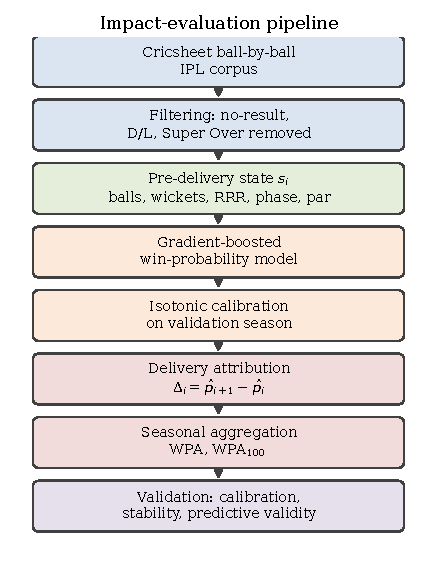
\includegraphics[width=\columnwidth]{fig_pipeline.pdf}
\caption{End-to-end architecture of the win probability instrument.}
\label{fig:pipeline}
\end{figure}

% =====================================================================
\section{Experimental Setup}
\label{sec:setup}

\subsection{Temporal Splitting}

All splits are performed \emph{at the match level and chronologically}.
Splitting at the delivery level would place highly correlated rows on
both sides of the partition and produce severely optimistic estimates.
Seasons 2007/08--2023 form the training set, 2024 the validation set,
and 2025--2026 the held-out test set. No test-season information is used
in feature construction, hyperparameter selection, or calibration.

\subsection{Effective Sample Size and Uncertainty}

Although the corpus contains 286{,}621 deliveries, the effective number
of independent outcome observations is approximately the number of
matches, 1{,}195. Every confidence interval in this paper is obtained by
bootstrap resampling \emph{of matches}, not of deliveries, with 500
replicates. We apply this without exception, including to the
descriptive analysis of Section~\ref{sec:res-h2h}, where it materially
changes what can be claimed.

\subsection{Evaluation Metrics}

Model quality is assessed with log loss, Brier score \cite{brier1950},
AUC-ROC, and expected calibration error (ECE) over 10 equal-frequency
bins, disaggregated by innings and phase. Rating quality is assessed by
\textbf{temporal stability}---Spearman rank correlation between a
player's rating in consecutive seasons, restricted to players qualifying
in both, against the same statistic for the conventional
aggregates---and \textbf{predictive validity}, in which squad-level
ratings aggregated over the announced playing XI predict the following
season's match winners.

\subsection{Rating Basis}

Held-out metrics come from the temporally split model. Player ratings
must cover every season, so they are computed from \emph{out-of-fold}
win probabilities: five folds grouped by match, each fold's model
calibrated on a disjoint quarter of its own training matches. Every
delivery is therefore scored by a model that never saw its match
(out-of-fold log loss 0.548). Because folds are random across seasons
rather than chronological, a 2015 rating may be produced by a model that
has seen 2019 matches. This is appropriate for description but would not
be admissible for a forecasting claim.

\subsection{Implementation}

Experiments were implemented in Python 3.13 using pandas 3.0,
scikit-learn 1.6, XGBoost 3.4, and the SHAP library 0.52. Training was
performed on a 16-thread AMD Ryzen 7 PRO 6850U laptop; total wall-clock
time for the full pipeline from a cold start is approximately 50
minutes. Code, cached model artefacts and derived rating tables are
available at \ph{repository URL}.

% =====================================================================
\section{Results}
\label{sec:results}

\subsection{The Instrument}
\label{sec:res-instrument}

Table~\ref{tab:wp} reports held-out performance for the win probability
model and both baselines.

\begin{table}[htbp]
\caption{Win Probability Model Performance on Held-Out Test Seasons}
\label{tab:wp}
\centering
\begin{tabular}{lcccc}
\toprule
\textbf{Model} & \textbf{Log loss} & \textbf{Brier} & \textbf{AUC} & \textbf{ECE} \\
\midrule
Resource-based \cite{dl1998} & 0.5638 & 0.1894 & 0.794 & 0.067 \\
Logistic regression          & 0.5033 & 0.1696 & 0.829 & 0.038 \\
GBM (raw)                    & 0.5201 & 0.1766 & 0.815 & \textbf{0.032} \\
GBM (isotonic, 1 season)     & 0.5319 & 0.1806 & 0.813 & 0.054 \\
GBM (isotonic, pooled)       & 0.5211 & 0.1766 & 0.814 & \textbf{0.032} \\
\bottomrule
\end{tabular}
\\[2pt]\footnotesize 95\,\% CI (match-level bootstrap, $B=500$) for the
pooled-calibration model: log loss $[0.473, 0.577]$, AUC $[0.764, 0.857]$.
\end{table}

Both learned models beat the resource baseline decisively, by roughly
0.05 nats of log loss and 0.02--0.035 AUC. Between them, however, the
result is a draw that we report rather than dress up: the regularised
logistic regression edges the ensemble on log loss (0.503 versus 0.521)
and AUC (0.829 versus 0.814), and the confidence intervals overlap
almost entirely.

We read this as the first indication of the paper's theme. Twenty20 win
probability is close to a smooth monotone function of a few
quantities---projected score against par, wickets in hand, required
rate---and with roughly a thousand independent outcomes there is not
enough information to identify much beyond that. The binding constraint
is the data, not the model class. The ensemble is retained as the
instrument for the reasons given in Section~\ref{sec:method}: it is the
best-calibrated specification in the table, and the attribution and SHAP
analyses require its interaction structure. Table~\ref{tab:phase}
disaggregates its performance.

\begin{table}[htbp]
\caption{Test Log Loss by Innings and Phase}
\label{tab:phase}
\centering
\begin{tabular}{lccc}
\toprule
\textbf{Innings} & \textbf{Powerplay} & \textbf{Middle} & \textbf{Death} \\
\midrule
First  & 0.6537 & 0.6446 & 0.6186 \\
Second & 0.5187 & 0.3776 & 0.2088 \\
\bottomrule
\end{tabular}
\end{table}

The structure is what the game implies. First-innings loss barely
improves from powerplay to death (0.654 to 0.619), because without a
target the eventual result remains close to a coin flip however well the
innings is read. The second innings is different in kind: loss falls by
more than half (0.519 to 0.209) as the chase resolves. Almost all usable
information lives in the second innings, which is also where the largest
win-probability movements are generated---a fact that returns in
Section~\ref{sec:res-stability}.

\subsection{Consequence I: A Silent Model-Selection Failure}
\label{sec:res-ess}

\begin{figure}[htbp]
\centering
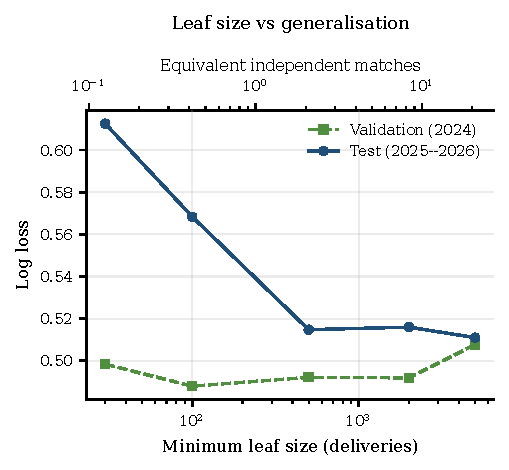
\includegraphics[width=\columnwidth]{fig_regularisation.pdf}
\caption{Minimum leaf size versus generalisation. The secondary axis rescales leaf size into equivalent independent matches. Validation loss is flat over the range across which test loss moves.}
\label{fig:regularisation}
\end{figure}

\begin{table}[htbp]
\caption{Effect of Minimum Leaf Size on Generalisation}
\label{tab:regularisation}
\centering
\begin{tabular}{rrccc}
\toprule
\textbf{Leaf} & \textbf{Matches} & \textbf{Val.\ LL} & \textbf{Test LL} & \textbf{Test AUC} \\
\midrule
30 & 0.1 & \textbf{0.4984} & 0.6125 & 0.761 \\
100 & 0.4 & \textbf{0.4880} & 0.5683 & 0.782 \\
500 & 2.1 & 0.4922 & 0.5148 & 0.816 \\
2000 & 8.3 & 0.4919 & 0.5160 & 0.817 \\
5000 & 20.8 & 0.5078 & \textbf{0.5110} & \textbf{0.827} \\
\bottomrule
\end{tabular}
\\[2pt]\footnotesize Leaf size in deliveries; ``Matches'' divides by the
$\approx$240 deliveries that share one outcome label. All models use
\texttt{n\_estimators} $=400$, \texttt{max\_depth} $=4$.
\end{table}

This is the paper's central result. The minimum-leaf hyperparameter is
specified in \emph{deliveries}, but the information content of the data
is measured in \emph{matches}. A leaf holding 30 deliveries---an
unremarkable default, and smaller than several libraries' own---holds
roughly one eighth of a single independent observation.

Table~\ref{tab:regularisation} and Fig.~\ref{fig:regularisation} show
the consequence. As the leaf grows from 30 to 5{,}000 deliveries, test
log loss falls from 0.613 to 0.511 and test AUC rises monotonically from
0.761 to 0.827: a 17\,\% reduction in loss obtained purely from
regularisation, with the curve flattening once leaves exceed roughly two
matches' worth of deliveries.

The validation curve, meanwhile, varies by less than 0.02 nats across
the entire range, and is \emph{minimised} at the two settings that
generalise worst. A practitioner following standard practice---tune on a
held-out season, select the lowest validation loss---would therefore
choose a model that is 20\,\% worse on the following two seasons, and
would receive no signal warning them of it. This is what we mean by a
silent failure: the diagnostic that is supposed to detect over-fitting
is itself computed on 71 independent outcomes, and is too noisy and too
close to the training regime to see it.

Two recommendations follow. First, regularisation hyperparameters for
ball-by-ball models should be specified in independent units---matches,
not deliveries---and grids floored accordingly; ours is floored at 500
deliveries for this reason. Second, validation for such models should
span multiple seasons or use grouped cross-validation over matches, so
that the effective sample size of the selection criterion is not itself
a handful of observations.

\subsection{Consequence II: Calibration}
\label{sec:res-calib}

\begin{figure}[htbp]
\centering
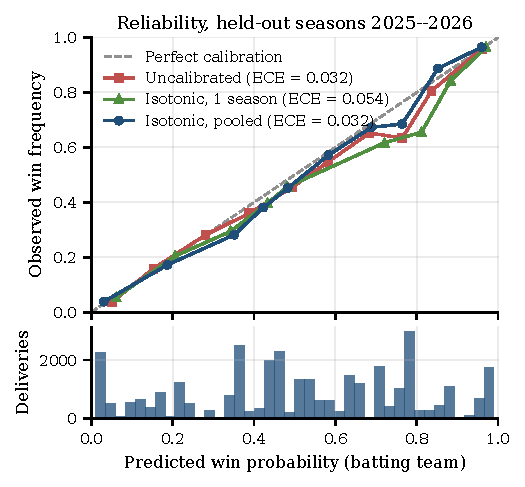
\includegraphics[width=\columnwidth]{fig_reliability.pdf}
\caption{Reliability diagram for the ensemble uncalibrated, calibrated on one season, and calibrated on pooled out-of-fold predictions, with the density of predictions beneath.}
\label{fig:reliability}
\end{figure}

The same cause corrupts the post-hoc calibration step. Fitting isotonic
regression on the validation season alone---Variant A of
Section~\ref{sec:method-calib}, and the textbook recipe---makes
calibration \emph{worse}, raising ECE from 0.032 to 0.054 and log loss
from 0.520 to 0.532. With 71 independent outcomes the monotone map
over-fits, and the corresponding curve in Fig.~\ref{fig:reliability}
visibly departs from the diagonal in the upper range. Pooling out-of-fold
training predictions with the validation season, Variant B, restores ECE
to 0.032.

Two things are worth noting. The uncalibrated ensemble tracks the
diagonal closely to begin with, with a mild optimism in the 0.6--0.85
band; its ECE of 0.032 is the lowest of the five specifications in
Table~\ref{tab:wp}, better than the logistic baseline's 0.038 despite
that model's superior log loss. And post-hoc calibration is therefore
neutral at best here: the honest summary is that it cannot help a model
that is already calibrated, and that fitted on too few independent
outcomes it will actively hurt.

\subsection{Consequence III: Rating Stability}
\label{sec:res-stability}

\begin{table}[htbp]
\caption{Season-over-Season Spearman Rank Correlation of Player Ratings}
\label{tab:stability}
\centering
\begin{tabular}{lcc}
\toprule
\textbf{Metric} & \textbf{Batters} & \textbf{Bowlers} \\
\midrule
Batting average / Bowling average & 0.193 & 0.106 \\
Strike rate / Economy rate & \textbf{0.413} & \textbf{0.480} \\
WPA & 0.143 & 0.144 \\
WPA$_{100}$ & 0.133 & 0.107 \\
\bottomrule
\end{tabular}
\\[2pt]\footnotesize $n=560$ batter and $n=534$ bowler consecutive-season
pairs, qualification threshold 120 deliveries.
\end{table}

The third consequence appears once the model's outputs are aggregated
into a player rating. WPA is markedly \emph{less} stable
season-over-season than the conventional rate statistics: strike rate
reaches a rank correlation of 0.413 for batters against 0.133 for
WPA$_{100}$, roughly three times as stable, and for bowlers economy rate
reaches 0.480 against 0.107, a factor of four and a half. WPA is
comparable to the traditional \emph{averages}, which are themselves
weakly persistent.

Two mechanisms operate here and they must be kept distinct, because they
have opposite implications for whether the problem is fixable.

The first is effective sample size again, now at player level. A
qualification threshold of 120 deliveries does not deliver 120
observations' worth of information, because win-probability movement is
heavily concentrated: second-innings death overs are 10.0\,\% of all
deliveries but carry 17.9\,\% of total $|\Delta|$ mass, a mean of 0.027
win-probability points per ball against 0.015 across the corpus. A
player's seasonal rating is dominated by a handful of decisive events,
so its sampling variance is far larger than the delivery count suggests.
This component is a statistical problem, and hierarchical shrinkage
toward role-specific priors would mitigate it.

The second is not a statistical artefact at all. Whether a player is on
strike or holding the ball at those decisive moments depends on batting
order, match situation and captaincy---circumstance, not skill---and
circumstance does not persist across seasons the way an ability does.
No amount of shrinkage recovers a signal that is not there.

The practical consequence is the same under either mechanism, and it is
a real limitation on what this class of metric can be used for. WPA
remains a defensible \emph{descriptive} account of what a player
contributed to matches already played. It is not, on this evidence, a
superior basis for \emph{projecting} future contribution, which is what
retention and auction decisions actually require.

\subsection{Consequence IV: Validation Power}

\begin{table}[htbp]
\caption{Next-Season Match Outcome Prediction from Aggregated Squad Ratings}
\label{tab:validity}
\centering
\begin{tabular}{lcc}
\toprule
\textbf{Rating basis} & \textbf{AUC [95\% CI]} & \textbf{Log loss} \\
\midrule
Conventional metrics & 0.528 [0.437, 0.616] & 0.6929 \\
WPA & 0.540 [0.440, 0.640] & 0.6937 \\
Combined & 0.524 [0.433, 0.609] & 0.6931 \\
\bottomrule
\end{tabular}
\\[2pt]\footnotesize Evaluated on 140 test-season matches.
\end{table}

The fourth consequence concerns the design of validation experiments
rather than of models. No rating basis separates next-season match
outcomes better than chance: every interval in
Table~\ref{tab:validity} comfortably contains 0.5, and the three
specifications are indistinguishable. WPA's nominal 0.540 is not a
positive finding.

The correct reading is underpowered rather than disproved, and the
arithmetic is the point. A test season supplies 140 independent matches;
the resulting bootstrap half-width is approximately 0.09 AUC. Any true
effect of prior-season squad quality on a single Twenty20 match is
plausibly well inside that band---IPL squads are deliberately equalised
by auction and retention rules, and one match is close to a coin flip
regardless. The experiment as designed could not have detected the
effect it was built to detect, and reporting the null without that
arithmetic would invite the wrong conclusion. Resolving the question
needs more independent matches: pooling several leagues, or a
rolling-origin design over all nineteen seasons rather than two.

\subsection{Model Interpretability}

\begin{figure}[htbp]
\centering
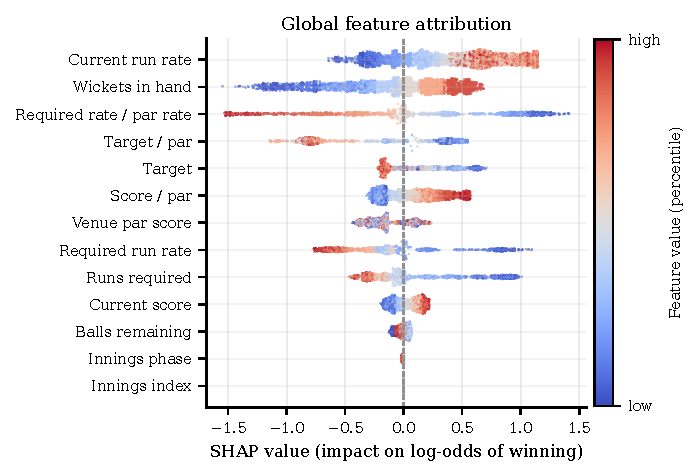
\includegraphics[width=\columnwidth]{fig_shap_summary.pdf}
\caption{Global feature attribution for the win probability model, features ordered by mean absolute SHAP value.}
\label{fig:shap}
\end{figure}

\begin{figure}[htbp]
\centering
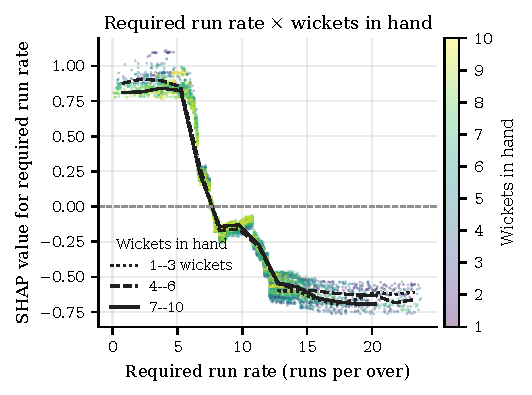
\includegraphics[width=\columnwidth]{fig_shap_dependence.pdf}
\caption{Interaction between required run rate and wickets in hand, with median trends by wicket band.}
\label{fig:shapdep}
\end{figure}

Having reported four ways the instrument can mislead, we check that it
is measuring the right thing. Fig.~\ref{fig:shap} ranks the drivers of
win probability by mean absolute SHAP value: current run rate (0.496),
wickets in hand (0.363), par-relative required run rate (0.323) and
par-relative target (0.307) dominate, followed by the absolute target
(0.212) and par-relative score (0.206). The directions are as cricketing
intuition requires---high current run rate and abundant wickets push the
log-odds up, high required rates push them down. Two features are
near-inert: innings phase (0.004) and the innings index itself (0.000).
The latter is not a defect but a consequence of the encoding: the
missingness pattern of the target and required-rate features already
identifies the innings perfectly.

The three par-relative features together account for more attributed
mass than their absolute counterparts (0.836 against 0.505), confirming
that the era normalisation of Section~\ref{sec:data} does real work.

Fig.~\ref{fig:shapdep} plots the interaction the attribution logic most
depends on. The required-run-rate contribution falls steeply and
monotonically, crossing zero at approximately 8 runs per over---close to
the par scoring rate---and flattening beyond about 13, by which point
the chase is effectively decided. The wicket bands separate at the high
end, but in the opposite direction to the intuition usually offered: at
required rates above 13, teams with 7--10 wickets in hand receive a
\emph{more} negative contribution from the required rate than teams with
1--3. This is not a paradox. When few wickets remain, the wickets
feature has already absorbed most of the bad news, leaving the required
rate less to explain. The joint effect on win probability is monotone in
the sensible direction; it is the \emph{decomposition} that shifts.

\subsection{Illustrative Case Study}

\begin{figure}[htbp]
\centering
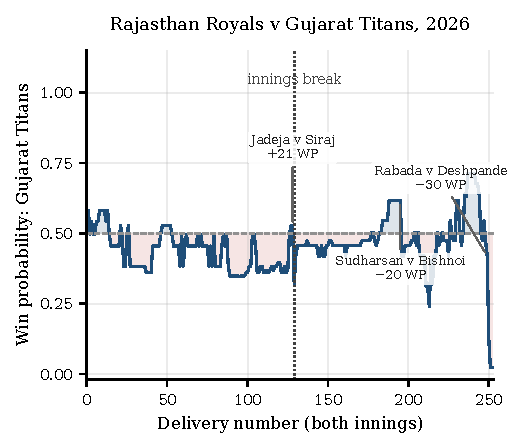
\includegraphics[width=\columnwidth]{fig_wp_trace.pdf}
\caption{Ball-by-ball win probability trace for Rajasthan Royals versus Gujarat Titans, Ahmedabad, 2026, a held-out test match.}
\label{fig:trace}
\end{figure}

Fig.~\ref{fig:trace} traces a close held-out match. Gujarat Titans' win
probability oscillates around even money for almost the entire contest,
crossing 0.5 repeatedly through both innings before collapsing to 0.02
on the final delivery.

Three deliveries carry the largest swings. Jadeja's strike against Siraj
at the end of the first innings is worth $+20.7$ win-probability points
because it lands at the innings boundary where the target is finally
fixed---a contribution the scorecard records as a handful of runs among
two hundred. Sai Sudharsan's dismissal by Bishnoi costs 19.8 points, and
Rabada's over to Deshpande in the closing stages swings 29.8 points back
against the chase. The allocation is instructive precisely where it
departs from the scorecard: a late over conceding few runs but arriving
with the match in the balance outranks an economical spell bowled while
the result was never in doubt. Economy rate cannot express that
distinction; a win-probability metric prices it directly.

\subsection{Divergence from Conventional Metrics}

\begin{table}[htbp]
\caption{Largest Rank Divergence Between WPA and Strike Rate, Season 2026}
\label{tab:divergence}
\centering
\begin{tabular}{lccc}
\toprule
\textbf{Player} & \textbf{Conv. rank} & \textbf{WPA rank} & \textbf{$\Delta$} \\
\midrule
KL Rahul & 11 & 50 & $-39$ \\
RA Jadeja & 49 & 14 & $+35$ \\
TM Head & 14 & 47 & $-33$ \\
D Ferreira & 10 & 40 & $-30$ \\
FH Allen & 2 & 32 & $-30$ \\
\bottomrule
\end{tabular}
\\[2pt]\footnotesize Positive $\Delta$: WPA ranks the player higher than
strike rate does. Qualification threshold 120 deliveries faced.
\end{table}

That the two families of metric disagree is not in doubt: among
qualified 2026 batters the largest rank shifts exceed thirty places in a
field of roughly sixty. Table~\ref{tab:divergence} shows the pattern is
dominated by high strike-rate players whom WPA demotes, while Jadeja, a
middle-order accumulator ranked 49th on strike rate, rises to 14th on
impact. The bowling side shows clearer role logic: Deshpande rises 35
places and Rabada 28 relative to their economy ranks, both death-overs
specialists whose economy is inflated by the phase they operate in,
while spinners Suyash Sharma and Shami fall 34 and 30 places from
economy ranks earned largely in the middle overs.

Two cautions are required, both following from
Section~\ref{sec:res-stability}. A single season's ranking is itself a
high-variance quantity, so individual rows should be read as
illustrative rather than as findings about those players. And a
divergence between WPA and conventional statistics is not evidence of
mispricing---it may equally reflect WPA's higher variance. We therefore
claim only that the two families rank players very differently, and in a
manner that tracks role, and we leave valuation to work that can join
ratings to prices.

\subsection{What Aggregation Buys, and Where It Stops}
\label{sec:res-h2h}

\begin{table}[htbp]
\caption{Chennai Super Kings Head-to-Head Record and Mean Per-Match WPA Decomposition}
\label{tab:h2h}
\centering
\begin{tabular}{lrrrr}
\toprule
\textbf{Opp.} & \textbf{M} & \textbf{Win \%} & \textbf{Bat WPA} & \textbf{Bowl $-$ Bat} \\
\midrule
MI & 41 & 48.8 [34, 63] & -0.046 & -0.066 to +0.242 \\
RCB & 35 & 60.0 [43, 77] & -0.007 & -0.093 to +0.282 \\
DC & 33 & 63.6 [48, 79] & +0.047 & -0.147 to +0.168 \\
RR & 32 & 50.0 [31, 69] & -0.019 & -0.099 to +0.204 \\
PBKS & 31 & 48.4 [31, 65] & +0.028 & -0.263 to +0.118 \\
KKR & 30 & 66.7 [50, 83] & +0.076 & -0.139 to +0.145 \\
SRH & 24 & 62.5 [42, 79] & +0.068 & -0.196 to +0.149 \\
\midrule
\textbf{All} & 259 & 56.0 [50, 62] & +0.011 & -0.026 to +0.084 \\
\bottomrule
\end{tabular}
\\[2pt]\footnotesize Brackets are 95\% match-level bootstrap intervals
($B=500$). Opponents with fewer than 20 fixtures are omitted as
underpowered. Per-match WPA is denominated in win probability, so a
team's total is close to $+0.5$ when it wins and $-0.5$ when it loses;
the batting/bowling split is the informative quantity, and the final
column gives the interval for that difference.
\end{table}

The natural response to everything above is to aggregate until the
effective sample size is adequate. This subsection asks how far that
gets, using the most favourable case available: Chennai Super Kings, the
most-capped franchise in the competition, with 259 completed fixtures
across nineteen seasons.

Two things are genuinely gained. The decomposition is \emph{exact}: by
the identity of Section~\ref{sec:method} a team's batting and bowling
contributions sum to its result, so the question "was this record built
with bat or ball?" is well posed in a way no combination of strike rate
and economy rate makes it. And the aggregate quantities are, marginally,
resolvable. CSK's overall win rate is 56.0\,\% with a 95\,\% interval of
$[49.8, 62.0]$, and their mean per-match bowling WPA of $+0.042$
$[+0.002, +0.085]$ excludes zero while their batting WPA of $+0.011$
$[-0.031, +0.053]$ does not.

It is exactly here that the analysis must stop, and the reason is
instructive. That bowling WPA is distinguishable from zero while batting
WPA is not does \emph{not} license the conclusion that bowling
contributes more: that is the difference-of-significance fallacy. The
quantity the claim requires is the difference itself, and it is
$+0.030$ with a 95\,\% interval of $[-0.026, +0.084]$. The interval
contains zero. Over 259 matches and nineteen seasons, the most-capped
franchise in the league does not supply enough independent observations
to establish which discipline wins its matches. We had drafted the
opposite claim before computing the interval, and record that here
because the error is an easy one to make.

The per-opponent rows make the same point more starkly.
Table~\ref{tab:h2h} and Fig.~\ref{fig:h2h} show that every individual
rivalry interval straddles the null: no head-to-head win rate is
distinguishable from even, and no batting-versus-bowling difference is
distinguishable from zero. Five further opponents are omitted entirely
with fewer than 20 fixtures. The point estimates are suggestive---CSK's
weakest record is against Mumbai Indians and their strongest against
Kolkata Knight Riders---but they are point estimates over thirty-odd
matches, and the intervals say so.

\begin{table}[htbp]
\caption{Leading Career WPA Contributors for Chennai Super Kings}
\label{tab:cskplayers}
\centering
\begin{tabular}{lrr}
\toprule
\textbf{Player} & \textbf{Deliveries} & \textbf{Career WPA} \\
\midrule
R Ashwin & 2{,}373 & $+2.13$ \\
DJ Bravo & 3{,}050 & $+1.83$ \\
M Muralitharan & 888 & $+1.82$ \\
MM Sharma & 1{,}020 & $+1.57$ \\
MS Dhoni & 3{,}354 & $+1.49$ \\
RA Jadeja & 4{,}720 & $+1.44$ \\
\bottomrule
\end{tabular}
\\[2pt]\footnotesize Deliveries faced plus deliveries bowled while
representing the franchise; minimum 240. Career totals aggregate over far
more deliveries than a seasonal rating, but remain subject to the
leverage concentration of Section~\ref{sec:res-stability}.
\end{table}

Table~\ref{tab:cskplayers} lists the franchise's leading career
contributors, and illustrates what the metric does well when it is used
descriptively. Five of the six are bowlers or bowling all-rounders.
Muralitharan is the sharpest illustration of leverage weighting: he
accumulates the third-highest career total from 888 deliveries, under a
third of Jadeja's 4{,}720, because his contributions arrived
disproportionately at decisive moments. No conventional aggregate ranks
a player above teammates with five times the workload. We present this
as a description of what occurred, not as an estimate of ability.

\begin{figure*}[t]
\centering
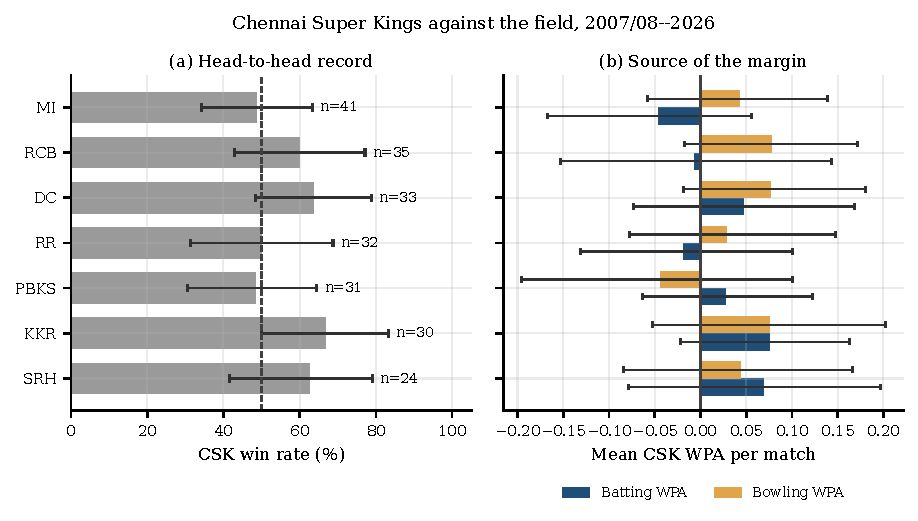
\includegraphics[width=\textwidth]{fig_h2h_csk.pdf}
\caption{Chennai Super Kings against the field, 2007/08--2026, opponents with at least 20 fixtures. (a) Head-to-head win rate with 95\,\% match-level bootstrap intervals; every interval straddles 50\,\%. (b) The same records decomposed into mean per-match batting and bowling WPA with the same intervals. The decomposition is exact, but 259 matches are not enough to resolve it.}
\label{fig:h2h}
\end{figure*}

% =====================================================================
\section{Discussion}
\label{sec:discussion}

\subsection{Implications for Practice}

The recommendations that follow are cheap to adopt and, on this
evidence, consequential.

\emph{Count independent outcomes before choosing hyperparameters.}
Regularisation expressed in rows is meaningless when rows are not
observations. Divide the nominal count by the cluster size and grid
accordingly; in our case a floor of 500 deliveries per leaf, about two
matches, was the difference between 0.61 and 0.51 test log loss.

\emph{Do not trust a single held-out season.} Validation loss over 71
independent outcomes was flat across a range where test loss moved by a
fifth, and pointed the wrong way. Use several seasons, or grouped
cross-validation over matches, and treat validation loss differences
smaller than the noise floor as absent.

\emph{Calibrate on enough independent outcomes, or not at all.} A
post-hoc calibrator is a fitted model and obeys the same arithmetic.
Ours degraded a well-calibrated ensemble when fitted on one season and
was neutral when fitted on a thousand outcomes.

\emph{Report intervals on descriptive statistics too.} The head-to-head
analysis of Section~\ref{sec:res-h2h} would have carried an attractive
and false headline had we not bootstrapped it. Descriptive work is not
exempt.

For player evaluation specifically, the position we end at is narrower
than the one this class of metric is usually asked to occupy. A
win-probability rating is a good descriptive instrument: it prices each
delivery by its effect on the quantity teams care about, it decomposes
exactly at team level, and it recovers role structure that economy rate
and strike rate obscure. It is not, on this evidence, a better
forward-looking valuation input than the conventional aggregates, whose
stability---whatever their context blindness---is their genuine virtue.

\subsection{Limitations}
\label{sec:limits}

\emph{Single competition.} Every result here comes from one league. The
mechanism we describe is arithmetic rather than cricketing, and we
expect it wherever labels are shared within a contest, but that
expectation is an argument rather than a demonstration. Replication on
other Twenty20 competitions, and on other sports with possession- or
pitch-level data, is the obvious next test.

\emph{Attribution granularity.} Run-outs and fielding contributions are
not attributed to the responsible fielder, so defensive value is omitted
from player ratings.

\emph{Extras convention.} Wides and no-balls are credited wholly against
the bowler with no offsetting batter credit. This is defensible for
wides but questionable for no-balls, which the batter does face; the
convention depresses batting WPA slightly at player level, and is why
Section~\ref{sec:res-h2h} uses the raw increment instead.

\emph{Opponent quality.} The state representation excludes team and
player identity, so a rating absorbs the quality of opposition faced.
The head-to-head decomposition inherits this.

\emph{Non-striker and partnership effects.} Credit accrues only to the
striker, so a non-striker who rotates strike or absorbs pressure
receives none.

\emph{Regime shift.} The par-relative features substantially mitigate
two decades of scoring inflation but do not eliminate it; the temporal
split measures the residual rather than removing it.

\emph{Rating basis.} Player ratings use out-of-fold probabilities whose
folds are random across seasons, which is appropriate for description
but inadmissible for forecasting.

\subsection{Future Work}

The most direct extension is more independent matches: pooling several
Twenty20 competitions would address the power limitation of
Section~\ref{sec:res-h2h} directly, and would test whether the
model-selection failure reproduces at larger effective sample sizes or
is specific to this regime. Hierarchical shrinkage of player ratings
toward role-specific priors would mitigate the sampling component of the
stability problem, though not the circumstantial component, and the gap
between those two is itself worth measuring. Fielder-level attribution
and opponent adjustment would improve the instrument. Finally, the
team-level decomposition generalises immediately to a full league-wide
matrix, of which Section~\ref{sec:res-h2h} presents one row---with the
caveat that, on the evidence here, most cells of that matrix will not be
resolvable either.

% =====================================================================
\section{Conclusion}

Ball-by-ball sports data invites a mistake that its file format makes
almost automatic: treating the delivery as the unit of observation. In
the Indian Premier League record, 286{,}621 deliveries carry 1{,}195
independent outcomes, and the factor of 240 between those numbers
propagates into every stage of a modelling pipeline.

We documented four consequences using a calibrated win-probability model
as the instrument. Model selection fails silently: an unregularised
ensemble records the best validation loss and generalises 20\,\% worse,
with validation loss flat across the range over which test loss moves.
Post-hoc calibration fitted on a single season degrades a
well-calibrated model, raising expected calibration error from 0.032 to
0.054. A leverage-concentrated rating is three to four times less
persistent season-over-season than strike rate, because 10.0\,\% of
deliveries carry 17.9\,\% of all win-probability movement. And a
validation design with 140 test matches cannot resolve the effects it
was built to detect.

Aggregation helps but does not rescue. The team-level decomposition is
exact by construction, and for the most-capped franchise in the league
the aggregate margin is marginally resolvable---yet 259 matches across
nineteen seasons still cannot establish whether that margin is built
with bat or ball, the difference being $+0.030$ with an interval of
$[-0.026, +0.084]$.

None of this argues against win-probability methods, which remain the
right way to price a delivery by what it does to the result, and which
recover role structure that aggregate statistics cannot express. It
argues that the number of rows in a ball-by-ball file is not the number
of things one has observed, and that regularisation, validation,
calibration and reporting should all be specified in the units that
actually carry information.

% =====================================================================
\begin{thebibliography}{00}

\bibitem{kish1965} L. Kish, \emph{Survey Sampling}. New York: Wiley, 1965.

\bibitem{field2007} C. A. Field and A. H. Welsh, ``Bootstrapping
clustered data,'' \emph{Journal of the Royal Statistical Society:
Series B}, vol. 69, no. 3, pp. 369--390, 2007. doi: \href{https://doi.org/10.1111/j.1467-9868.2007.00593.x}{10.1111/j.1467-9868.2007.00593.x}.

\bibitem{roberts2017} D. R. Roberts et al., ``Cross-validation
strategies for data with temporal, spatial, hierarchical, or
phylogenetic structure,'' \emph{Ecography}, vol. 40, no. 8,
pp. 913--929, 2017. doi: \href{https://doi.org/10.1111/ecog.02881}{10.1111/ecog.02881}.

\bibitem{lindsey1963} G. R. Lindsey, ``An investigation of strategies in
baseball,'' \emph{Operations Research}, vol. 11, no. 4, pp. 477--501, 1963.

\bibitem{tango2007} T. Tango, M. Lichtman, and A. Dolphin, \emph{The
Book: Playing the Percentages in Baseball}. Potomac Books, 2007.

\bibitem{yurko2019} R. Yurko, S. Ventura, and M. Horowitz, ``nflWAR: A
reproducible method for offensive player evaluation in football,''
\emph{Journal of Quantitative Analysis in Sports}, vol. 15, no. 3,
pp. 163--183, 2019.

\bibitem{cervone2016} D. Cervone, A. D'Amour, L. Bornn, and K. Goldsberry,
``A multiresolution stochastic process model for predicting basketball
possession outcomes,'' \emph{Journal of the American Statistical
Association}, vol. 111, no. 514, pp. 585--599, 2016.

\bibitem{decroos2019} T. Decroos, L. Bransen, J. Van Haaren, and
J. Davis, ``Actions speak louder than goals: Valuing player actions in
soccer,'' in \emph{Proc. 25th ACM SIGKDD Int. Conf. Knowledge Discovery
and Data Mining}, 2019, pp. 1851--1861.

\bibitem{dl1998} F. C. Duckworth and A. J. Lewis, ``A fair method for
resetting the target in interrupted one-day cricket matches,''
\emph{Journal of the Operational Research Society}, vol. 49, no. 3,
pp. 220--227, 1998.

\bibitem{stern2016} S. E. Stern, ``The Duckworth--Lewis--Stern method:
Extending the Duckworth--Lewis methodology to deal with modern scoring
rates,'' \emph{Journal of the Operational Research Society}, vol. 67,
no. 12, pp. 1469--1480, 2016. doi: \href{https://doi.org/10.1057/jors.2016.30}{10.1057/jors.2016.30}.

\bibitem{bailey2006} M. Bailey and S. R. Clarke, ``Predicting the match
outcome in one day international cricket matches, while the game is in
progress,'' \emph{Journal of Sports Science and Medicine}, vol. 5,
no. 4, pp. 480--487, 2006.

\bibitem{davis2015} J. Davis, H. Perera, and T. B. Swartz, ``A simulator
for Twenty20 cricket,'' \emph{Australian \& New Zealand Journal of
Statistics}, vol. 57, no. 1, pp. 55--71, 2015. doi: \href{https://doi.org/10.1111/anzs.12109}{10.1111/anzs.12109}.

\bibitem{lemmer2002} H. H. Lemmer, ``The combined bowling rate as a
measure of bowling performance in cricket,'' \emph{South African Journal
for Research in Sport, Physical Education and Recreation}, vol. 24,
no. 2, pp. 37--44, 2002.

\bibitem{chen2016} T. Chen and C. Guestrin, ``XGBoost: A scalable tree
boosting system,'' in \emph{Proc. 22nd ACM SIGKDD Int. Conf. Knowledge
Discovery and Data Mining}, 2016, pp. 785--794.

\bibitem{lundberg2017} S. M. Lundberg and S.-I. Lee, ``A unified
approach to interpreting model predictions,'' in \emph{Advances in
Neural Information Processing Systems 30}, 2017, pp. 4765--4774.

\bibitem{brier1950} G. W. Brier, ``Verification of forecasts expressed
in terms of probability,'' \emph{Monthly Weather Review}, vol. 78,
no. 1, pp. 1--3, 1950.

\bibitem{platt1999} J. Platt, ``Probabilistic outputs for support vector
machines and comparisons to regularized likelihood methods,'' in
\emph{Advances in Large Margin Classifiers}, MIT Press, 1999,
pp. 61--74.

\bibitem{niculescu2005} A. Niculescu-Mizil and R. Caruana, ``Predicting
good probabilities with supervised learning,'' in \emph{Proc. 22nd Int.
Conf. Machine Learning}, 2005, pp. 625--632.

\bibitem{cricsheet} S. Rushe, ``Cricsheet: Ball-by-ball data for cricket
matches,'' accessed 2 September 2026. [Online]. Available:
https://cricsheet.org

\bibitem{kumar2018} J. Kumar, R. Kumar, and P. Kumar, ``Outcome
prediction of ODI cricket matches using decision trees and MLP
networks,'' in \emph{Proc. 1st Int. Conf. Secure Cyber Computing and
Communication}, 2018, pp. 343--347. doi: \href{https://doi.org/10.1109/ICSCCC.2018.8703301}{10.1109/ICSCCC.2018.8703301}.

\bibitem{vistro2019} D. M. Vistro, F. Rasheed, and L. G. David, ``The
cricket winner prediction with application of machine learning and data
analytics,'' \emph{Int. J. Scientific and Technology Research}, vol. 8,
no. 9, pp. 985--990, 2019.

\bibitem{saikia2013} H. Saikia, D. Bhattacharjee, and A. Bhattacharjee,
``Performance based market valuation of cricketers in IPL,''
\emph{Sport, Business and Management: An International Journal}, vol. 3,
no. 2, pp. 127--146, 2013. doi: \href{https://doi.org/10.1108/20426781311325069}{10.1108/20426781311325069}.

\bibitem{sharma2013} S. K. Sharma, ``A factor analysis approach in
performance analysis of T-20 cricket,'' \emph{Journal of Reliability and
Statistical Studies}, vol. 6, no. 1, pp. 69--76, 2013.

\end{thebibliography}

\end{document}
